	\documentclass[10pt,oneside]{CBFT_book}
	% Algunos paquetes
	\usepackage{amssymb}
	\usepackage{amsmath}
	\usepackage{graphicx}
% 	\usepackage{libertine}
% 	\usepackage[bold-style=TeX]{unicode-math}
	\usepackage{lipsum}

	\usepackage{natbib}
	\setcitestyle{square}

	\usepackage{polyglossia}
	\setdefaultlanguage{spanish}


	\usepackage{CBFT.estilo} % Cargo la hoja de estilo

	% Tipografías
	% \setromanfont[Mapping=tex-text]{Linux Libertine O}
	% \setsansfont[Mapping=tex-text]{DejaVu Sans}
	% \setmonofont[Mapping=tex-text]{DejaVu Sans Mono}

	%===================================================================
	%	DOCUMENTO PROPIAMENTE DICHO
	%===================================================================

\begin{document}

% =================================================================================================
\chapter{Fenómenos dependientes del tiempo}
% =================================================================================================

% =================================================================================================
\section{Ley de Faraday e inducción}
% =================================================================================================

En un circuito $\Gamma$ se induce una fuerza electromotriz (fem) dada por
\[
	\mathcal{E} = \int_\Gamma \vb{E}\cdot d\vb{\ell}
\]
y por otra parte
\[
	\int_\Gamma \vb{E}\cdot d\vb{\ell} = - k \: \dtot{}{t}\left( \int_S \vb{B}\cdot d\vb{S} \right)
\]
donde el signo menos es la ley de lenz; la fem se opone el cambio de flujo.
Esta propiedad no puede depender de que exista o no circuito.
Si el circuito permanece rígido, la derivada temporal pasa directamente adentro como derivada
parcial y se tiene
\[
	\int_\Gamma \vb{E}\cdot d\Bell = - k \: \left( \int_S \dpar{\vb{B}}{t} \cdot d\vb{S} \right)
\]
la cual, por aplicación del teorema de Stokes en una superficie que englobe al circuito,
conduce a
\[
	\int_S \rotorm{E} \cdot d\vb{S} = - k \: \left( \int_S \dpar{\vb{B}}{t} \cdot d\vb{S} \right),
\]
o bien
\[
	\rotorm{E} = -\frac{1}{c} \dpar{\vb{B}}{t},
\]
que nos dice que si en un punto hay variación temporal de \vb{B} se está produciendo un
campo \vb{E} no conservativo.

\[
	\mathcal{E} = -\frac{1}{c} \frac{d}{dt}\left( \int_S \vb{B}\cdot d\vb{S} \right)
\]
siendo $S=\partial\Gamma$ y donde 
\[
	\mathcal{E} = \int_\Gamma \vb{E}\cdot d\vb{\ell}
\]
siendo \vb{E} un campo irrotacional medido en el frame donde $\Gamma$ está en reposo.
El signo menos es la ley de lenz, la FEM se opone el cambio de flujo.

Pero la variación de flujo puede deberse a variación de \vb{B} o a deformación del circuito.
\[
	\frac{d}{dt}\int_S \vb{B}\cdot d\vb{S} = \int_S \dpar{\vb{B}}{t}\cdot d\vb{S} +
	\int_\Gamma \vb{B}\times\vb{V} \cdot d\vb{\ell}
\]
y entonces
\[
	\int_\Gamma \vb{E}'\cdot d\vb{\ell} = -\frac{1}{c} \int_S \dpar{\vb{B}}{t}\cdot d\vb{S} +
	\frac{1}{c} \int_\Gamma \vb{B}\times\vb{V} \cdot d\vb{\ell}
\]
\[
	\int_\Gamma [\vb{E}'- \vb{B}\times\vb{V} ] \cdot d\vb{\ell} = -\frac{1}{c} \int_S \dpar{\vb{B}}{t}\cdot d\vb{S}
\]
y si $\vb{E} = \vb{E}'- \vb{B}\times\vb{V}$ es el campo medido en el laboratorio se llega a la 
ley de Faraday,
\[
	\int_\Gamma \vb{E}\cdot d\vb{\ell} = -\frac{1}{c} \int_S \dpar{\vb{B}}{t}\cdot d\vb{S}
\]
y usando el teorema de Stokes a su forma diferencial
\[
	\rotorm{E} = -\frac{1}{c} \dpar{\vb{B}}{t}
\]
siendo este campo \vb{E} claramente no conservativo.

\subsection{Corrección a las ecuaciones}

Entonces resultan las siguientes cuatro ecuaciones
\[
	\divem{D} = 4 \pi \rho \qquad \qquad \rotorm{E} = -\frac{1}{c} \dpar{\vb{B}}{t}
\]
que son las leyes de Coulomb y Faraday en forma diferencial. Asimismo
\[
	\divem{B} = 0 \qquad \qquad \rotorm{H} = \frac{4\pi}{c} \vb{J}
\]
que es la no existencia de monopolos magnéticos y la ley de Ampere. En el último caso con $\divem{J}=0$
que es para corrientes estacionarias.

Justamente por ello la ecuación relacionada con la ley de Ampere está incompleta así puesto que se dedujo
para corrientes estacionarias. Maxwell introduce la continuidad aproximadamente en 1865.
Entonces, como 
\[
	\divem{J} + \dpar{\rho}{t } = 0 
\]
se sigue que 
\[
	\divem{J} + \frac{\partial}{\partial t} \frac{\divem{D}}{4\pi} =
	\Nabla\cdot\left[ \vb{J} + \frac{1}{4\pi} \dpar{\vb{D}}{t} \right] = 0
\]
que es posible pensar como una nueva densidad de corriente \vb{J}. 
Entonces la ley de Ampere completa es:
\[
	\rotorm{H} = \frac{4\pi}{c} \vb{J} + \frac{1}{c}\dpar{\vb{D}}{t}
\]
siendo $\partial\vb{D}/\partial t$ la llamada corriente de desplazamiento. 
Las cuatro ecuaciones están ahora completas y constituyen las {\it ecuaciones de Maxwell}.

Estas ecuaciones son lineales de manera que vale superposición para ellas. No obstante no vale
superposición para campos relacionados no linealmente con $\vb{D}, \vb{E}, \vb{H}$ y $\vb{B}$.

\subsection{Potenciales}

Entonces, para campos dinámicos el conjunto de ecuaciones es
\be
	\divem{D} = 4 \pi \rho \qquad \qquad \rotorm{E} = -\frac{1}{c} \dpar{\vb{B}}{t}
	\label{maxwell_e}
\ee
\be
	\divem{B} = 0 \qquad \qquad \rotorm{H} = \frac{4\pi}{c} \vb{J} + \frac{1}{c}\dpar{\vb{D}}{t}
	\label{maxwell_m}
\ee
Dado que $\divem{B} = 0$ al igual que en magnetostática, podemos derivar \vb{B} del potencial 
vector \vb{A}. Luego veremos que persistirá una indeterminación de la $\divem{A}$. 
No obstante, como \vb{E} no tiene rotor nulo, entonces no existe $\phi$ potencial escalar.
En efecto, tomando
\[
	\rotorm{E} + \frac{1}{c}\dpar{\vb{D}}{t} = 
	\rotorm{E} + \frac{\partial}{\partial t}\left( \frac{1}{c} 
	\rotorm{A}\right) = \Nabla\times\left[ \vb{E} + \frac{1}{c}\dpar{\vb{A}}{t}\right] = 0
\]
podemos pensar en un potencial general $\Phi$ tal que 
\[
	- \Nabla \Phi = \vb{E} + \frac{1}{c}\dpar{\vb{A}}{t}
\]
o bien 
\[
	\vb{E}  = -\Nabla \Phi - \frac{1}{c}\dpar{\vb{A}}{t},
\]
donde por supuesto $\Phi$ no tiene significado de trabajo, medido independientemente de la
trayectoria, como sí lo tenía el potencial electrostático.

Podemos expresar las ecuaciones de Maxwell \eqref{maxwell_e} y \eqref{maxwell_m} en
términos de estos potenciales $\vb{A},\Phi$,
\[
	\divem{E} = 4\pi\rho \rightarrow 
	\Nabla\cdot\left( -\Nabla \Phi - \frac{1}{c}\dpar{\vb{A}}{t} \right) = 4\pi\rho
\]
\[
	\rotorm{B} - \frac{1}{c}\dpar{E}{t} =  \frac{4\pi}{c} \vb{J}  \rightarrow
	\Nabla\times(\rotorm{A}) - \frac{1}{c}\frac{\partial}{\partial t}\left( 
	-\Nabla \Phi - \frac{1}{c}\dpar{\vb{A}}{t} \right)=  \frac{4\pi}{c}\vb{J}
\]
de manera que resultan dos ecuaciones para los potenciales, pero acopladas
\[
	\nabla^2 \Phi + \frac{1}{c} \frac{\partial}{\partial t}\divem{A} = -4 \pi \rho
\]
\[
	\nabla^2 \vb{A} - \frac{1}{c^2} \dpar[2]{\vb{A}}{t} -\Nabla \left( \divem{A} + \frac{1}{c}
	\dpar{\Phi}{t} \right) = -\frac{4\pi}{c} \vb{J}
\]
Así como están son de difícil resolución.

\subsubsection{Cambio de Gauge}

Podemos desacoplarlas utilizando la arbitrariedad de los potenciales
\be
	\rotorm{A} = \vb{B} \qquad -\Nabla\Phi - \frac{1}{c} \dpar{\vb{A}}{t} = \vb{E}
	\label{ecs_potencial_em}
\ee
si le sumamos una función al potencial vector,
\[
	\vb{A} \rightarrow \vb{A}'= \vb{A} + \Nabla \Lambda,
\]
se da que 
\[
	\rotorm{A} = \rotorm{A'}
\]
pero
\[
	- \Nabla\Phi - \frac{1}{c}\dpar{\vb{A}}{t} - \frac{1}{c}\dpar{\Nabla\Lambda}{t} = \vb{E}
\]
lo cual vale si y sólo si
\[
	-\Nabla\left( \Phi + \frac{1}{c} \dpar{\Lambda}{t} \right) -\frac{1}{c}\dpar{\vb{A}}{t}   = \vb{E}
\]
de manera que requiero 
\[
	\Phi \rightarrow \Phi'= \Phi - \frac{1}{c} \dpar{\Lambda}{t}
\]
y estas dos ecuaciones fijan la transformación de gauge. Como con $\vb{A'}, \Phi'$ siguen valiendo las 
\eqref{ecs_potencial_em}, requiero que 
\[
	\divem{A'} + \frac{1}{c}\dpar{\Phi'}{t} = 0 = \divem{A} + \frac{1}{c}\dpar{\Phi}{t} + \nabla^2 \Lambda
	- \frac{1}{c^2} \dpar[2]{\Lambda}{t}
\]
entonces
\[
	\divem{A} + \frac{1}{c}\dpar{\Phi}{t} = -\left(\nabla^2 \Lambda - \frac{1}{c^2} \dpar[2]{\Lambda}{t}\right)
\]
y si usamos los nuevos potenciales, ahora sin apóstrofes para no confundir con notación redundante,
\[
	\nabla^2 \vb{A} - \frac{1}{c^2}\dpar[2]{\vb{A}}{t} = -\frac{4\pi}{c}\vb{J}
\]
\[
	\nabla^2 \Phi - \frac{1}{c^2}\dpar[2]{\Phi}{t} = -\frac{4\pi}{c}\rho
\]
ambos potenciales satisfacen sendas ecuaciones de onda no homogéneas. 
Los potenciales son como ondas propagándose en el espacio y luego se verá que los campos también
serán algo parecido.
El {\it gauge} de Lorentz o ``condición de Lorentz'' es
\[
	\divem{A} + \frac{1}{c} \dpar{\Phi}{t} = 0.
\]
En este caso resulta una ecuación de onda para $\Lambda$ de manera que habrá muchísimos $\Lambda$
que nos dan el mismo campo. Infinitos potenciales dan el mismo campo.

Podemos imponer también 
\[
	\divem{A} = 0
\]
el {\it gauge} de Coulomb y entonces
\[
	\nabla^2 \Phi = -4\pi\rho
\]
vemos que el potencial $\phi$ cumple la ecuación de Poisson.
No obstante, veremos luego que la condición de Lorentz es invariante relativista mientras
que la de Coulomb no lo es.
El campo se describirá como el electrostático, que es estacionario, de manera que
\[
	\dpar{\Phi}{t} = 0
\]
y entonces
\[
	\divem{A} + \frac{1}{c} \dpar{\Phi}{t} = 0
\]
siendo cada uno de los términos nulos por sí mismo.
El gauge, la ``medida'' describe a los potenciales, pero los resultados físicos deben ser
independientes del gauge.

% =================================================================================================
\section{Conservación de la energía (teorema de Poynting)}
% =================================================================================================

Sea una región $V$ con volumen fijo, en la cual existen \vb{E}, \vb{B} variantes con el tiempo y
ninguna otra cosa. Parece lógico suponer que se puede escribir una ecuación de continuidad para
$U$ la densidad de energía electromagnética por unidad de volumen.
La fuerza por unidad de volumen de los campos sobre las cargas es
\[
	\vb{F} = q \left( \vb{E} + \frac{1}{c} \pv{v}{B} \right)
\]
entonces
\[
	\delta W = \vb{F}\cdot d\vb{\Bell} = q \vb{E}\cdot d\vb{\Bell}, 
\]
dado que \vb{B} no hace trabajo por ser perpendicular la fuerza a la velocidad.
\[
	\delta U = q \:\vb{E}\cdot d\vb{\Bell} 
\]
Para una carga $q$ es
\[
	\dtot{U}{t} = q \: \vb{E}\cdot \vb{v} 
\]
y para una distribución de cargas,
\[
	\dtot{U}{t} = \int_V \rho \vb{E}\cdot \vb{v} \: dV = \int_V \vb{J}\cdot \vb{E} \: dV
\]
que no es otra cosa que la potencia entregada por los campos \vb{E}, \vb{B} dentro del volumen
$V$. Es una conversión de energía electromagnética en energía mecánica o térmica.

\[
	\int_V \vb{J}\cdot \vb{E} dV = \int_V \left[ \frac{c}{4\pi}(\rotorm{H})\cdot\vb{E} - 
		\frac{1}{4\pi}\dpar{\vb{D}}{t}\cdot\vb{E} \right] dV
\]
Si usamos la identidad
\[
	\Nabla\cdot(\pv{E}{H}) = \vb{H}\cdot(\rotorm{E}) - \vb{E}\cdot(\rotorm{H}),
\]
podemos escribir
\[
	= \int_V \frac{c}{4\pi} \left( \left[ \vb{H}\cdot(\rotorm{E}) - \Nabla\cdot(\pv{E}{H}) \right] - 
		\frac{1}{4\pi}\dpar{\vb{D}}{t}\cdot\vb{E}  \right) dV
\]
\[
	= - \frac{1}{4\pi}\int_V \left[ \vb{H}\cdot\dpar{\vb{B}}{t} + \dpar{\vb{D}}{t}\cdot\vb{E} \right] dV - 
		\int_V \frac{c}{4\pi}  \Nabla\cdot(\pv{E}{H}) dV
\]
\notamargen{Acá hay un par de tricks que hay que explicar, de como extraer la derivada temporal, etc.}
\[
	= - \frac{1}{8\pi}\frac{d}{dt} \int_V \left[ \vb{H}\cdot\vb{B} + \vb{D}\cdot\vb{E} \right] dV - 
		 \frac{c}{4\pi} \int_S (\pv{E}{H}) dS
\]
siendo $S\equiv\partial V$. Si denominamos ahora
\[
	\vb{S} \equiv \frac{c}{4\pi}(\pv{E}{H}) \qquad \text{vector de Poynting}
\]
\[
	U = \frac{1}{8\pi}\left( \vb{H}\cdot\vb{B} + \vb{D}\cdot\vb{E} \right) \qquad \text{Densidad de energía EM}
\]
resulta que 
\[
	\pe{J}{E} = -\dpar{U}{t} - \divem{S},
\]
entonces hemos hallado una ecuación de continuidad con $U, \vb{S}$ en función de los campos, que nos
dice que la conservación de la energía por unidad de volumen es
\[
	\dpar{U}{t} = -\divem{S} -\pe{J}{E}.
\]
Integrando esta ecuación resulta
\[
	\int_V \dpar{U}{t} dV + \int_V \divem{S} dV = - \int_V \pe{J}{E} dV = -\int_S \vb{S}\cdot d\vb{S}
\]
donde se ha aplicado el teorema de Gauss en el miembro derecho.
\notamargen{Si cambia la energía en el volumen $V$ es debido a que se transfiere energía a las
cargas como $\pe{E}{J}$ o se escapa energía electromagnética como flujo de \vb{S}.}
Así
\[
	\int_V \dpar{U}{t} dV + \int_V \divem{S} dV = -\int_S \vb{S}\cdot d\vb{S}
\]
siendo el primer término del LHS la variación de la energía total, el segundo la potencia entregada por
los campos sobre las fuentes y el RHS el flujo de energía a través de la región transportado por el
vector de Poynting.
Notemos que $\pe{J}{E}$ es el trabajo hecho por unidad de tiempo y por volumen por los campos.
Localmente la conservación de la energía es
\[
	\dtot{U_{cam}}{t} + \dtot{U_{mec}}{t} = -\int_S \vb{S}\cdot d\vb{S},
\]
donde la integral del miembro derecho es la energía que escapa a través de una región (menos el flujo
del vector de Poynting).
Los campos \vb{S} y $U$ no están relacionados linealmente con \vb{E} y \vb{H}.

% =================================================================================================
\section{Conservación del momento. Tensor de Maxwell}
% =================================================================================================

La idea es que una onda plana puede portar momento pero no momento angular.
Una onda electromagnética circularmente polarizada puede transportar momento angular.
Se tiene
\[
	\dtot{\vb{P}_{cam}}{t} + \dtot{\vb{P}_{mec}}{t} = \int_S \: T \: \hat{n} dS
\]
y el miembro derecho refleja el momento lineal que se escapa por la superficie de
integración.
La versión integral de la anterior es
\[
	\dtot{}{t} \int_V \: \vb{g} \: dV + \dtot{}{t} \int_V \: \vb{p} \: dV = \int_S \: T \: \hat{n} dS
\]
que refleja la conservación del momento lineal. El primer término del lhs es el momento
lineal del campo electromagnético, mientras que el segundo representa las fuerzas sobre
las cargas en volumen.

Acometeremos primeramente la segunda integral del lado izquierdo.
En el discreto se tiene
\[
	\vb{F} = \dtot{\vb{P}}{t} = q\vb{E} + q\frac{1}{c} \pv{v}{B} 
\]
y pasando al continuo
\[
	\dtot{\vb{P}_M}{t} = \int_V \left[ \rho\vb{E} + \frac{1}{c} \pv{J}{B}  \right] dv
\]
y si suponemos MLIH se puede expresar la densidad de carga en términos de la divergencia
del campo $\vb{D}$ y así
\[
	\dtot{\vb{P}_M}{t} = \int_V \left[ \frac{1}{4\pi} (\divem{D}) \vb{E} + 
	\frac{1}{c} \left( \frac{c}{4\pi}\rotorm{H} - \frac{1}{4\pi}\dtot{\vb{D}}{t} \right) 
	\times \vb{B} \right] dv
\]
\[
	\dtot{\vb{P}_M}{t} = \int_V \left[ \frac{1}{4\pi} (\divem{D}) \vb{E} +  
	\frac{1}{4\pi} (\Nabla\times\vb{H}\times\vb{B}) - \frac{1}{4\pi c}\dtot{\vb{D}}{t} 
	\times \vb{B} \right] dv
\]
Ahora, usando las siguientes cuentas auxiliares
\[
	\dpar{}{t}(\pv{D}{B}) = \dpar{\vb{D}}{t}\pv{}{B} + \pv{D}{}\dpar{\vb{B}}{t}
\]
\[
	\epsilon\mu \: \dpar{}{t}(\pv{E}{H}) = \epsilon\mu \: \dpar{\vb{D}}{t}\pv{}{B} + 
	\epsilon\mu\pv{D}{}\dpar{\vb{B}}{t}
\]
y ahora volviendo
\[
	\dtot{\vb{P}_M}{t} = \frac{1}{4\pi} \int_V \left[  (\divem{D}) \vb{E} + (\Nabla\times\vb{H}\times\vb{B}) 
	-\frac{\epsilon\mu}{c} \left( \dpar{}{t}(\pv{E}{H}) - \pv{E}{}\dpar{\vb{H}}{t} \right) \right] dv	
\]
haciendo un pase de miembros y expresando \vb{H} en términos de \vb{E} es
\begin{multline*}
	\dtot{\vb{P}_M}{t} + \frac{\epsilon\mu }{4\pi c} \int_V \dpar{}{t}(\pv{E}{H}) dV = \\
	\frac{1}{4\pi} \int_V \left[  (\divem{D}) \vb{E} - \epsilon \pv{E}{}(\Nabla\times\vb{E}) +
	\rotorm{H}\times\vb{B} + \vb{H}(\divem{B}) \right] dV	 
\end{multline*}
donde el último término en el integrando del RHS es cero y se lo puedo sumar por ello.
Esto es para lograr un término simétrico en los campos eléctrico y magnético.
Prosiguiendo
\begin{multline*}
	\dtot{\vb{P}_M}{t} + \frac{\epsilon\mu }{4\pi c} \dtot{}{t}\int_V (\pv{E}{H}) dV = \\
	\frac{1}{4\pi} \int_V \left[  (\divem{D}) \vb{E} - \pv{D}{}(\Nabla\times\vb{E}) +
	\vb{H}(\divem{B}) - \vb{B}(\rotorm{H}) \right] dV	
\end{multline*}
donde la segunda integral del lhs define a
\[
	\vb{g} = \frac{\mu \epsilon}{4\pi} (\pv{E}{H}) = \frac{\vb{S}}{v^2}
\]
siendo $v$ la velocidad de la onda en el medio.
\notamargen{Tenía anotado: ``transferencia de impulso lineal de los campos a las cargas''.}
Podemos utilizar un identidad más, ver Apéndice ID4, para expresar
\[
	\vb{D}\times(\rotorm{E}) = \frac{1}{2} \Nabla(\pe{E}{D}) - (\vb{E}\cdot\nabla)\vb{D}
\]
y así obtener
\[
	\Nabla \cdot[ \vb{E}\vb{D} - \frac{1}{2} \: \mathbb{1} \: (\pe{D}{E}) ],
\]
donde debe notarse que el primer producto $\vb{E}\vb{D}$ es un producto tensorial, no es un
número su resultado sino un tensor (que vendrá representado como una matriz).
Se puede hacer lo propio con el campo magnético y al final del día se tendrá
\begin{multline*}
	\dtot{\vb{P}_M}{t} + \frac{1}{c} \dtot{}{t}\int_V \vb{g} \: dV = \\
	\frac{1}{4\pi} \int_V \Nabla\left( \left[ \vb{D}\vb{E} - 
	\frac{1}{2}\mathbb{1}( \pe{D}{E}) \right] + 
	\left[ \vb{H}\vb{B} - \frac{1}{2}\mathbb{1}(\pe{H}{B}) \right] \right) dV
\end{multline*}
% \[
% 	= \frac{1}{4\pi} \int_V \Nabla\left( \left[ \vb{D}\vb{E} - \frac{1}{2}\mathbb{1}( \pe{D}{E}) \right] + 
% 		\left[ \vb{H}\vb{B} - \frac{1}{2}\mathbb{1}(\pe{H}{B}) \right] \right) dV
% \]
donde los primeros términos dentro de cada corchete son productos tensoriales.
Aplicando el teorema de la divergencia en el rhs, y expresando la derivada de la integral
de $\vb{g}$ con el momento de los campos, se puede escribir
\be
	\dtot{\vb{P}_M}{t} + \dtot{\vb{P}_{C}}{t}  =
	\frac{1}{4\pi} \int \: \vb{D}\vb{E} + \vb{H}\vb{B}
	- \frac{1}{2} \: \mathbb{1} \left[ \: \pe{D}{E} + \pe{H}{B} \: \right] \: d\vb{S}
\ee


Hemos encontrado que se puede definir la conservación como flujo de un tensor de segundo rango,
\[
	T_{ik} = \frac{1}{4\pi}\left[ \epsilon E_iE_k + \mu H_iH_k - \frac{1}{2}\delta_{ik}
	( \epsilon E^2 + \mu H^2)\right]
\]
que es el tensor de esfuerzos de Maxwell. El tensor da entonces flujo de momento. Si el
medio es LIH el tensor es simétrico.
El tensor de Maxwell dinámico es la suma de los tensores estáticos eléctrico y magnético
a la vez.

Entonces
\[
	\int_V (\rho\vb{E} + \frac{1}{c}(\pv{J}{B}) ) dV + 
	\dtot{}{t}\left( \frac{1}{4\pi c}\int_V (\pv{D}{B})dV\right) = \int_S T \cdot d\vb{S}
\]
con la normal saliente. Luego, localmente la conservación del momento lineal es
\[
	\dtot{\vb{P}_{mec}}{t} + \dtot{\vb{P}_{cam}}{t}  = \int_S T \cdot d\vb{S}
\]
donde el RHS es la fuerza por unidad de área a través de $S$ que actúa sobre las partículas y
los campos dentro de $V$.
Definiendo
\[
	\frac{1}{c^2} \vb{S}=  \vb{g} = \frac{1}{4\pi c}(\pv{D}{B})
\]
se tiene que \vb{g} es una densidad de flujo de momento y también puede expresarse
\[
	\vb{g} = \frac{\epsilon\mu}{4\pi c}(\pv{E}{H}).
\]

Observemos que el tensor de Maxwell es un tensor cartesiano.

\begin{ejemplo}{\bf Problema 10b}

El problema está relacionado con lo ilustrado bajo estas líneas

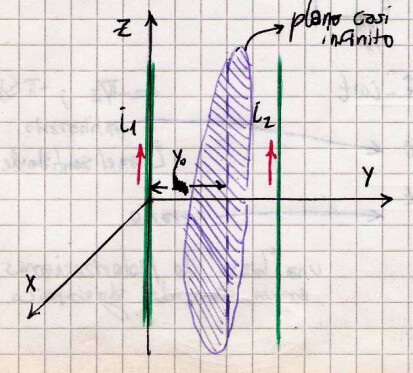
\includegraphics[width=0.3\textwidth]{images/fig_ft1_problema10bA.jpg}

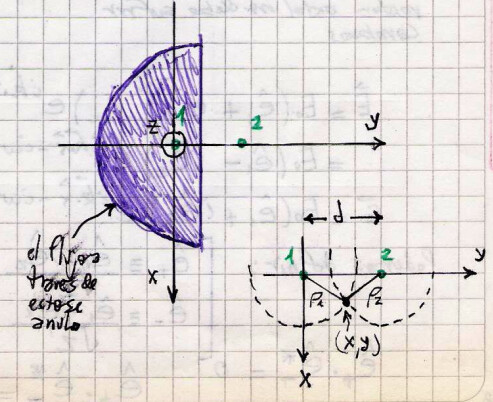
\includegraphics[width=0.3\textwidth]{images/fig_ft1_problema10bB.jpg}

Los campos y los ángulos involucrados son
\[
	\vb{B}_1 = \frac{2}{c \rho_1 } I_1 \: \hat{e}_{\vp_1} \qquad \qquad 
	\vb{B}_2 = \frac{2}{c \rho_2 } I_2 \: \hat{e}_{\vp_2}
\]
\[
	\cos\vp_1 = \frac{x}{\rho_1} \qquad \sin\vp_1 = \frac{y}{\rho_1} \qquad 
	\cos\vp_2 = \frac{x}{\rho_2} \qquad \sin\vp_2 = \frac{y-d}{\rho_1} 
\]
\[
	\rho_1 = \sqrt{ x^2 + y^2 } \qquad \hat{e}_{\vp_1} = \cos\vp_1 \:\yver - \sin\vp_1 \:\xver
\]
\[
	\rho_1 = \sqrt{ x^2 + (y-d)^2 } \qquad 
	\hat{e}_{\vp_2} = \cos\vp_2 \:\yver - \sin\vp_2 \:\xver
\]
 
Calcularemos el tensor de Maxwell (será genérico)
\[
	\vb{B} = \vb{B}_1 + \vb{B}_2 \qquad \qquad B_z=0
\]
luego como $\nver = (n_x,n_y,0)$ es
\[
	T = \frac{1}{8\:\pi}\begin{pmatrix}
	        B_x^2 - B_y^2  & 2 B_x B_y & 0 \\
		2 B_x B_y  & B_y^2 - B_x^2  & 0 \\
		0	& 0	& B_z^2 - B_x^2 - B_y^2
	       \end{pmatrix}	
\]
\[
	T \cdot \nver |_y = (T\cdot\nver)\cdot\yver =
	\frac{1}{8\:\pi} \left[ 2B_xB_y n_x - ( B_y^2 - B_x^2 ) n_y\right]
\]
Me interesa solamente la componente en $\yver$ dado que las otras serán nulas.
La dirección $\nver$ es la saliente en el semicilindro infinito.

El producto escalar tiene metido $B_1, B_2$ lo cual generará términos con $B_1$,
términos con $B_2$ y términos acoplados.
Lo que depende de $B_1$ es como una autofuerza y debería ser nula (es antifísica).
Vemos la parte de interacción solamente (términos mezclados).
Lo que depdnde solamente de $B_2$ tampoco lo consideramos.

Luego,
\[
	B_{y_1} B_{y_2} = \frac{4 J_1 J_2}{c^2} \frac{y_0}{x^2 + y_0^2} 
	\frac{y_0-d}{(\sqrt{x^2+ (y_0-d)^2})^2}
\]
\[
	B_{x_1} B_{x_2} = \frac{4 J_1 J_2}{c^2} 
	\frac{x}{x^2 + y_0^2} \frac{x}{(x^2+ (y_0-d)^2)}
\]
\[
	F_y = \int\int (T\cdot\nver)\cdot\yver \: dx \: dz
\]
definiendo un $f_y \equiv F_y/\text{Long.}$ se tendrá
\[
	f_y = \int_{-\infty}^\infty (T\cdot\nver)\cdot\yver \: dx =
	8 \frac{J_1 J_2}{c^2} \frac{-2\pi}{d} \frac{1}{8\pi} = - \frac{2I_1I_2}{c^2 d}
\]
y la última integral sale porque es {\it de esas} que están en tablas.
 
\end{ejemplo}

\begin{ejemplo}{\bf Problema 12b}

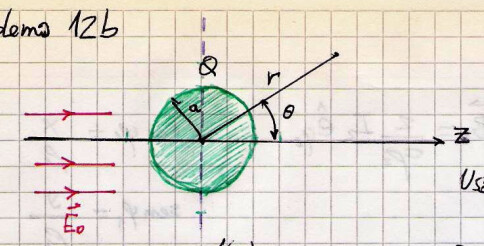
\includegraphics[width=0.3\textwidth]{images/fig_ft1_problema12bA.jpg}

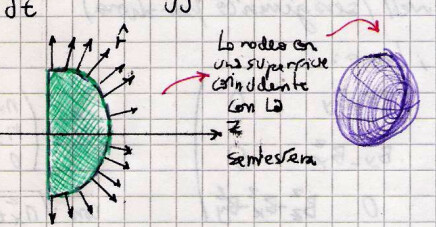
\includegraphics[width=0.3\textwidth]{images/fig_ft1_problema12bB.jpg}
 
\end{ejemplo}

\begin{ejemplo}{\bf Problema 14}

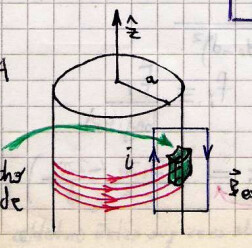
\includegraphics[width=0.3\textwidth]{images/fig_ft1_problema14A.jpg}

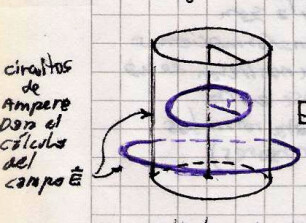
\includegraphics[width=0.3\textwidth]{images/fig_ft1_problema14B.jpg}

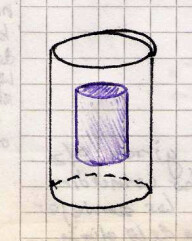
\includegraphics[width=0.25\textwidth]{images/fig_ft1_problema14C.jpg}
 
\end{ejemplo}





% =================================================================================================
\subsection{El tensor de Maxwell en acción}
% =================================================================================================

Se consideran sistemas interactuantes a distancia

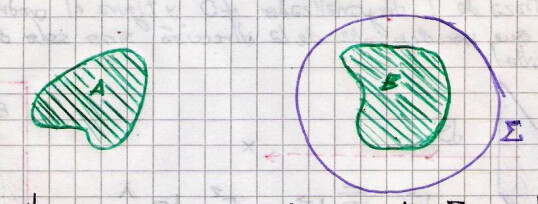
\includegraphics[width=0.3\textwidth]{images/fig_ft1_PicsMaxwellA.jpg}

y la idea es encerrar al cuerpo con una superficie cerrada $\Sigma$ lo que nos permitira conocer
el campo total sobre esa superficie.
Tenemos la siguiente ecuación que no sé bien que
\[
	F_i(b) = \int_V f_i(b) \: dV = \int_V \partial_j T_{ij} \: dV = \int_S T_{ij} \hat{n}_j dS.
\]

El tensor T será diagonal si una de las direcciones es paralela al campo. Con el T puede calcularse
la fuerza que hacen los campos \vb{E}, \vb{B} sobre una cierta distribución de cargas y corrientes,
con tal de evaluar su flujo en alguna superficie que las contenga (como se ve en la figura)

\begin{figure}[htb]
	\begin{center}
	\includegraphics[width=0.4\textwidth]{images/fig_ft1_maxwell.pdf}	 
	\end{center}
	\caption{}
\end{figure} 


y con tal de que 
\[
	\dtot{}{t}\left(\int_V \vb{g} dV \right) = 0 \qquad \qquad \vb{g} =  \frac{1}{4\pi c}(\pv{E}{B})
\]
puesto que en ese caso será
\[
	\vb{F} = \int_S T \cdot d\vb{S}.
\]

En este caso se suele definir el concepto de presión de radiación
\[
	\vb{R}_{rad} \equiv \dtot{\vb{F}}{S} T\cdot\hat{n}.
\]

T es un tensor con autovalores reales; coincidiendo sus autovectores con la dirección del campo.
Es independiente del sentido del campo, depende del valor absoluto de los mismos.
\[
	T_{ik} = \frac{1}{4\pi} \left[ \epsilon E_iE_k - \frac{1}{2}\delta_{ik} \epsilon E^2 \right] 
\]
es el tensor eléctrico y
\[
	T_{ik} = \frac{1}{4\pi} \left[ \mu H_iH_k - \frac{1}{2}\delta_{ik} \mu H^2  \right] 
\]
el tensor magnético.

\subsection{Ejemplos del tensor de Maxwell}

Respecto de la figura, donde vemos que el campo penetra en el recinto y la tensión es hacia adentro,
\begin{figure}[htb]
	\begin{center}
	\includegraphics[width=0.4\textwidth]{images/fig_ft1_tensorM1.pdf}
	\includegraphics[width=0.5\textwidth]{images/fig_ft1_tensorM2.pdf}	
	\end{center}
	\caption{}
\end{figure} 
escribimos 
\[
	d\vb{S} = -dS\hat{y} \qquad \vb{F}_{\text{sobre}\:-q} = -F\hat{y}
\]
\[
	T|_S = \begin{pmatrix}
	        -E_y^2	& 0 	& 0 \\
		0	& E_y^2	& 0 \\
		0	& 0	& -E_y^2
	       \end{pmatrix}
\]
la fuerza atractiva hacia afuera del recinto.
\begin{figure}[htb]
	\begin{center}
	\includegraphics[width=0.8\textwidth]{images/fig_ft1_tensorM3.pdf}	 
	\end{center}
	\caption{}
\end{figure} 

En este otro caso, el campo sale del recinto y la tensión es hacia afuera pués la $\hat{n}$
ha cambiado de sentido.
\[
	T\cdot d\vb{S} \propto \hat{y} \qquad \vb{F}_{\text{sobre}\:+q} = F\hat{y}
\]
es una fuerza atractiva hacia afuera del recinto.
\begin{figure}[htb]
	\begin{center}
	\includegraphics[width=0.4\textwidth]{images/fig_ft1_tensorM4.pdf}	 
	\end{center}
	\caption{}
\end{figure} 

Aquí abajo el campo es tangencial al recinto, la tensión penetra en él.

\begin{figure}[htb]
	\begin{center}
	\includegraphics[width=0.9\textwidth]{images/fig_ft1_tensorM5.pdf}	 
	\end{center}
	\caption{}
\end{figure} 

Se llega al concepto de T cuando pensamos en campos para justificar las interacciones.
Este concepto es válido también para el campo magnético.
Para medios materiales, lineales e isótropos, se tendrán consecuentemente los siguientes tensores
eléctrico y magnético estáticos [electro- y magneto-estáticos], respectivamente,
\[
	T_{ik} = \frac{1}{4\pi} \left[ E_iD_k - \frac{1}{2}\delta_{ik} \pe{D}{E}(1-b_e) \right] 
\]
\[
	T_{ik} = \frac{1}{4\pi} \left[ H_iB_k - \frac{1}{2}\delta_{ik} \pe{H}{B}(1-b_m)  \right] .
\]
Se definen la electrofricción y magnetofricción, $b_e,b_m$, respectivamente como
\[
	b_e = \frac{\rho}{\varepsilon} \dtot{\varepsilon}{\rho}  = \int_S T_{ij} n_j \: dS
\]
hallándose la $b_m$ con una definición análoga.
La fuerza total de este término es nula pero el efecto es tender a reventar el medio.

Para el vacío el $T_{ij}$ es simétrico y con elementos reales, por lo tanto es diagonalizable 
con autovalores reales.
Para diagonalizarlo podemos usar razonamientos físicos o matemáticos.

Cuando T está diagonalizado la traza no es nula y figura el cuadrado del campo eléctrico,
o sea que no depende de la dirección sino solo del valor absoluto de la intensidad.
Cuando se diagonaliza, haciendo
\[
	| T - \lambda \mathbb{1} | = 0
\]
se tienen $\lambda_1 = E^2 / 8\pi$ y $\lambda_{2,3} = - E^2 / 8\pi$, donde el
autovector de $\lambda_1$ corresponde a la dirección de \vb{E} y $\lambda_{2,3}$
a las direcciones perpendiculares.

El siguiente figurín ilustra

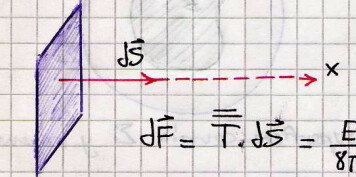
\includegraphics[width=0.3\textwidth]{images/fig_ft1_tensorMax_B.jpg}

donde se tiene
\[
	d\vb{F} = T d\vb{S} = \frac{E^2}{8\pi} dS \hat{e}_x,
\]
o bien en palabras; el campo $\vb{E}$ por unidad de área en la dirección de la normal a la superficie
por el elemento de superficie transmite una tensión a través de la superficie.

\begin{ejemplo}{}

Considerando el siguiente dibujo vemos que se quiere obtener la fuerza sobre $q$ para lo cual se
encierra la carga (con una semiesfera al infinito) y calcula el flujo resultante

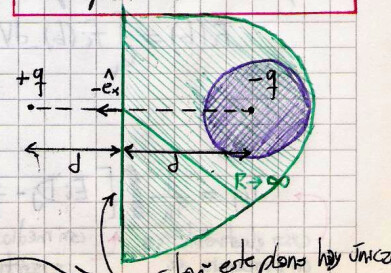
\includegraphics[width=0.3\textwidth]{images/fig_ft1_tensorMax_C.jpg}

Queda un plano sobre el cual solamente hay $E_x\hat{x}$.
Entonces
\[
	F_x = -\frac{4d^2q^2}{8\pi} \int_{\text{Plano xy}} \: \frac{dy dz}{( \: d^2 + y^2 + z^2 \: )^3} = 
	- \frac{q^2}{( 2 d )^2}.
\]
En este caso las dos cargas tienen signos opuestos. Sobre el plano el campo es perpendicular,
se transmite entonces una tensión a través del mismo plano; existe una fuerza atractiva.

Para dos cargas iguales

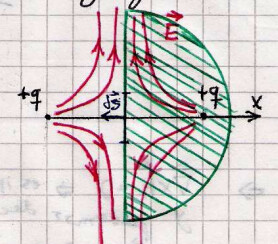
\includegraphics[width=0.3\textwidth]{images/fig_ft1_tensorMax_D.jpg}

se tiene en $x=0$
\[
	\vb{E} = \frac{ 2 q ( y \yver + z \zver )}{( d^2 + y^2 + z^2 )^{3/2}}
\]
el campo es paralelo al plano. Entonces la interacción es repulsiva porque se ejerce una presión a
través de $dS$ que empuja a $q$. El tensor es
\[
	T(0,y,z) = \frac{1}{4\pi}\begin{pmatrix}
	        -\frac{E^2}{2} & 0 & 0 \\
		0 & E_y^2 - \frac{E^2}{2} & E_y E_z \\
		0 & E_y E_z & E_z^2 - \frac{E^2}{2} 
	\end{pmatrix}
\]
Inmediatamente se llega, para la fuerza sobre la carga de la derecha, a
\[
	F_x = - \frac{q^2}{ 8 \pi } \int \frac{ 4 ( y^2 + z^2 ) }{( d^2 + y^2 + z^2 )^3} dy dz = 
	- q^2 \int_0^\infty \frac{ \rho^3 }{(d^2 + \rho^2)^3} d\rho = 
	\frac{q^2}{(2d)^2},
\]
que recupera el resultado de la ley de Coulomb (previo pasaje a cilíndricas de la integral
y buscando el resultado en una tabla).

\end{ejemplo}

\begin{ejemplo}{\bf Cables paralelos por los que circula corriente}

Se analizará fuerza por unidad de longitud dada la extensión infinita de los cables.

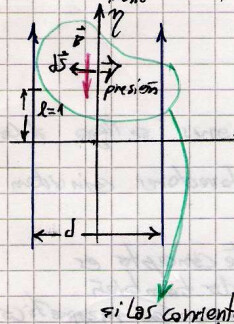
\includegraphics[width=0.3\textwidth]{images/fig_ft1_cablesParalelosCorriente.jpg}

\[
	\vb{B}(\eta) = \vb{B}^1(\eta) + \vb{B}^2(\eta) = - \frac{4I}{c} \frac{y}{(d/2)^2 + y^2} \xver
\]
Los cables se atraerán si las corrientes son paralelas. Los cables se repulsan si las
corrientes son antiparalelas (sentido contrario).

La siguiente figurita  ilustra

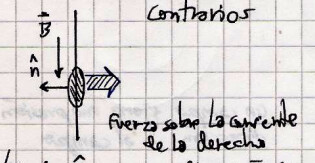
\includegraphics[width=0.25\textwidth]{images/fig_ft1_cablesParalelosCorrienteB.jpg}

que si cambio de normal $\hat{n}$ cambio dirección de la fuerza (debida al flujo del tensor
de Maxwell, no al flujo del campo que será nulo).
 
\end{ejemplo}

\begin{ejemplo}{\bf Fuerza en imán polar}

En este ejemplo se desprecia el flujo lateral y el interior (que es mucho más pequeño).
La ilustración muestra una pieza polar de imán.

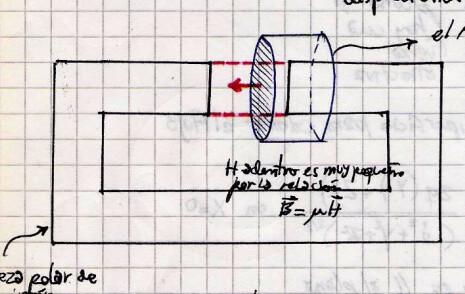
\includegraphics[width=0.4\textwidth]{images/fig_ft1_imanPolar.jpg}
 
Luego, el tensor es
\[
	T_{ij} = \frac{1}{4\pi} \left[ H_i B_j - \frac{1}{2} \delta_{ij} \vb{H}\cdot\vb{B} \right].
\]
 
\end{ejemplo}


\notamargen{Un campo ejerce una presión en una dirección perpendicular al campo.}
\[
	d\vb{F}|_{\parallel} = T\cdot d\vb{S}|_{\parallel} \rightarrow \frac{E^2}{8\pi} dS|_{\parallel}
\]
el campo eléctrico transmite una tensión $E^2/8\pi$ paralela a la dirección del campo.
El tensor diagonalizado es 
\[
	T = \frac{1}{4\pi}\begin{pmatrix}
	        E^2/2	& 0 	& 0 \\
		0	& -E^2/2	& 0 \\
		0	& 0	& -E^2/2
	       \end{pmatrix}
\]
En cambio, el tensor no diagonalizado es
\[
	T = \frac{1}{4\pi}\begin{pmatrix}
	        \frac{1}{2}( E_x^2 - E_y^2 -E_z^2 ) & E_x E_y	& E_x E_z \\
		E_x E_y	& \frac{1}{2}( E_y^2 - E_z^2 -E_x^2 ) & E_y E_z \\
		E_x E_z & E_y E_z & \frac{1}{2}( E_z^2 - E_x^2 -E_y^2 )
	       \end{pmatrix}
\]

Si se elige uno de los ejes a lo largo del campo $\vb{E}$ se diagonaliza el tensor, lo cual es
un razonamiento matemático.

% =================================================================================================
\section{Método cuasiestacionario}
% =================================================================================================

Se aproximan campos y fuentes con frecuencias bajas, es decir cuando $\omega \approx 0$, serán
campos que varían lentamente con el tiempo.
O sea que en alguna medida se utilizarán expresiones estáticas para una situación dinámica.
Observemos que se desarrollará la parte espacial pero la temporal quedará como está.
Se considera
\[
	\vb{E}(\vb{x},t) = \vec{\mathbb{E}} \euler^{i\omega/c \hat{n}\cdot\vb{x}} \euler^{-i\omega t}
\]
y se desarrollará la parte espacial en torno a $\omega=0$. Se hace un Taylor derivando con respecto
a $\omega$ y evaluando en $\omega=0$.
Comencemos el show,
\[
	\vb{E}(\vb{x},t) = \vec{\mathbb{E}} + \omega\frac{i\hat{n}\cdot\vb{x}}{c} \vec{\mathbb{E}} +
			\omega^2 \frac{i^2(\hat{n}\cdot\vb{x})^2}{c^2} \vec{\mathbb{E}}
\]
y si le {\it pegamos} la parte temporal será
\[
	\vb{E}(\vb{x},t) = \underbrace{ \vec{\mathbb{E}} \euler^{-i\omega t} }_{\vb{E}^{(0)}} + 
	\underbrace{\omega\frac{i\hat{n}\cdot\vb{x}}{c} \vec{\mathbb{E}}\euler^{-i\omega t}}_{\vb{E}^{(1)}} +
	\underbrace{\omega^2\frac{i^2(\hat{n}\cdot\vb{x})^2}{c^2}\vec{\mathbb{E}}\euler^{-i\omega t}}_{\vb{E}^{(2)}}
\]

Para el campo \vb{B} puede hacerse una descomposición análoga. 
Veamos cómo resulta esto aplicándolo a la ecuación del rotor del campo $\vb{E}$, es decir a
$\rotorm{E} = -1/c \: \partial{\vb{B}}/\partial t$.
Considerando hasta orden 2, se tienen
\[
	\rotorm{}(\vb{E}^0 + \vb{E}^1 + \vb{E}^2) = -\frac{1}{c} \dpar{}{t}(\vb{B}^0 + \vb{B}^1 + \vb{B}^2)
\]
\[
	0 + \underbrace{\rotorm{E}^1}_{\propto \omega } + \underbrace{\rotorm{E}^2}_{\propto \omega^2 } = 
	\underbrace{\frac{i\omega}{c}\vb{B}^0}_{\propto \omega } + \underbrace{\frac{i\omega}{c}
	\vb{B}^1}_{\propto \omega^2 } + \underbrace{\frac{i\omega}{c}\vb{B}^2}_{\propto \omega^3 }
\]
\[
	-\frac{1}{c}\dpar{\vb{B}}{t} = -\frac{1}{c}(-i\omega)\vec{\mathbb{B}}\euler^{-i\omega t}
	-\frac{1}{c}\omega(-i\omega)\frac{i\hat{n}\cdot\vb{x}}{c}\vec{\mathbb{B}}\euler^{-i\omega t}
	-\frac{1}{c}\frac{\omega^2}{2}(-i\omega)\frac{i^2(\hat{n}\cdot\vb{x})^2}{c^2}\vec{\mathbb{B}}\euler^{-i\omega t}
\]
\[
	-\frac{1}{c}\dpar{\vb{B}}{t} = \frac{i\omega}{c}\vb{B}^{(0)} 
	+ \frac{i\omega}{c} \underbrace{\frac{i\omega}{c}\vec{\mathbb{B}}\euler^{-i\omega t}}_{\vb{B}^{(1)}}
	+ \frac{i\omega}{c} \underbrace{ \left.\frac{\omega^2}{2}\frac{i^2(\hat{n}\cdot\vb{x})^2}	
	{c^2}\vec{\mathbb{B}} \euler^{-i\omega t}\right.}_{\vb{B}^{(2)}}
\]
Igualando miembro a miembro se establece una equivalencia entre órdenes,
\[
	\rotorm{E}^{(0)} = 0 \qquad \qquad \rotorm{E}^{(1)} = -\frac{1}{c}\dpar{\vb{B}^{(0)}}{t}
\]
donde el orden cero es el de los campos estáticos y el orden 1 es el término
cuasiestacionario. Notemos que no {\it cabalgan} en la misma medida \vb{E} y \vb{B},
como se aprecia de la ecuación del rotor para el orden 1 del campo eléctrico.

\begin{sidewaystable}
	%\centering A table
	\begin{center}
	\begin{tabular}{|c|c|c|}
	\hline
	Orden cero & Orden uno & Orden dos \\
	\hline
	& & \\
	$\displaystyle{ \divem{}\epsilon\vb{E}^0 = 4\pi\rho^0 }$ & $ \divem{}\epsilon\vb{E}^{(1)} = 4\pi\rho^{(1)} $ 
	& $ \divem{}\epsilon\vb{E}^{(2)} = 4\pi\rho^{(2)} $  \\
	& & \\
	$ \rotorm{}\vb{E}^{(0)} = 0 $ & $\displaystyle{\rotorm{}\vb{E}^{(1)} = -\frac{1}{c} \dpar{\vb{B}^{(1)}}{t} }$ 
	& $ \displaystyle{ \rotorm{}\vb{E}^0 = -\frac{1}{c} \dpar{\vb{B}^{(2)}}{t} }$  \\
	& & \\
	$ \divem{}\vb{B}^{(0)} = 0 $ & $\divem{}\vb{B}^{(1)} = 0  $ & $ \divem{}\vb{B}^{(2)} = 0 $  \\
	& & \\
	$ \displaystyle{ \rotorm{}\frac{1}{\mu}\vb{B}^{(0)} = \frac{4\pi}{c}\vb{J}^{(0)} } $ 
	& $ \displaystyle{ \rotorm{}\frac{1}{\mu}\vb{B}^{(1)} = \frac{4\pi}{c}\vb{J}^{(1)} + 
	\frac{1}{c}\dpar{\epsilon\vb{E}^{(0)}}{t} } $ 
	& $ \displaystyle{ \rotorm{}\frac{1}{\mu}\vb{B}^{(2)} = \frac{4\pi}{c}\vb{J}^{(2)} +
	\frac{1}{c}\dpar{\epsilon\vb{E}^{(1)}}{t} } $  \\
	& & \\
	$ \divem{}\vb{J}^{(0)} = 0 $ & $\displaystyle{ \divem{}\vb{J}^{(1)} = -\dpar{\rho^{(0)}}{t} }$ 
	& $\displaystyle{ \divem{}\vb{J}^{(2)} = -\dpar{\rho^{(1)}}{t} } $  \\
	& & \\
	\hline
	\end{tabular} 
	\end{center}  
	%\caption{A caption}
\end{sidewaystable}

Consideramos $\omega/c \ell \ll 1$ con $\ell$ alguna longitud característica del sistema.
Esta es la aproximación del sistema para poder usar cuasiestacionario.

En general, en el método cuasiestacionario se alternarán para un mismo campo el valor constante
(no necesariamente cero) y alguna función de $(\vb{x}, t)$. Es decir, que si $E_{par} = cte.$
entonces $E_{impar} \neq cte.$ y si $B_{impar} \neq cte.$ entonces $B_{par} = cte.$

No es muy formal decir $\omega$ chico puesto que no es adimensional. Débese comparar contra
alguna magnitud del problema físico, por ejemplo
\[
	\frac{\omega}{c} \ell \to 0
\]
es una buena magnitud característica, donde $\ell$ es una longitud característica del
sistema físico.

Para las densidades de carga y de corriente, $\rho,\vb{J}$ vale un desarrollo similar.
Recordemos que la nomenclatura de corrientes en 
\[
	\rotorm{H} = \frac{4\pi}{c}\vb{J} + \frac{1}{c}\dpar{\vb{D}}{t}
\]
es corriente de conducción y de desplazamiento respectivamente.

Cuando un conductor no es perfecto vale la ley de Ohm,
\[
	\vb{J} = \sigma \vb{E} \qquad  \delta = \frac{c^2}{2\pi\omega\sigma}
\]
donde $\delta$ es la profundidad pelicular, una longitud de penetración.


\begin{ejemplo}{\bf Problema 4}

La figura ilustra la situación, donde se considera $ a \gg h$ y se desprecian los bordes.

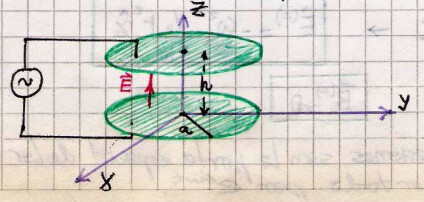
\includegraphics[width=0.4\textwidth]{images/fig_ft1_problema4_cuasiestac.jpg}

Se considera también que está alimentado con tensión y no con corriente. Luego, 
$ \omega /c \ell \to 0$ con $\ell$ cierta longitud característica.
Luego veremos quién es esta $\ell$.

Se trabaja cada uno de los órdenes.

{\bf Orden cero}. De las ecuaciones corresopndientes y por integración del campo estático
obtenemos
\[
	\int \vb{E}\cdot d\Bell = V_0,
\]
de modo que 
\[
	\vb{E}^{(0)} = \frac{V_0}{h} \zver \qquad \vb{B}^{(0)} = 0
\]

{\bf Orden uno}. Desde las ecuaciones de \vb{E}, que utilizan el $\vb{B}^{(0)}$ se obtiene
$\vb{E}^{(1)}=0$.
Utilizando las ecuaciones de $\vb{B}$, con la prescripción de $\vb{E}^{(0)}$ se llega a
\[
	\vb{B}^{(1)} = - i \left[ \frac{\omega r}{c} \right] \frac{V_0}{2h} \phiver
\]
donde $r < a$. De esta expresión se puede ver que el término entre corchetes involucra una
variable adimensional que nos puede servir de candidata para $\ell$. En efecto con $\ell \equiv a$
el radio del capacitor puede ser la longitud buscada.

La densidad $\sigma$ de cada placa es uniforme, dadas las aproximaciones, o lo que es lo mismo,
fluctúa muy rápidamente. Como $ \lambda \gg a $ entonces
\[
	\frac{\omega a}{c} \ll 1.
\]

{\bf Orden dos}. La ecuación del rotor del campo eléctrico es
\[
	\rotorm{E}^{(2)} = \Frac{\omega}{c}^2 \frac{V_0}{2h} r \phiver,
\]
lo cual conduce a 
\[
	\vb{E}^{(2)} = -\Frac{\omega}{c}^2 \frac{V_0}{4h} r^2 \zver \qquad \vb{B}^{(2)} = 0.
\]

Como vemos, se alterna qué campo es nulo en cada orden subsiguiente. Todas estas expresiones son
la parte espacial de los campos, faltando {\it pegarles} la parte temporal.

Se puede ver que el campo converge a una función de Bessel
\[
	\vb{E} = \vb{E}^{(0)} + \vb{E}^{(2)} + \vb{E}^{(4)} + ... =
	\frac{V_0}{h} \left[ 1 - \frac{1}{4} \Frac{\omega}{c}^2 r^2 + ...\right] =
	\frac{V_0}{h} J_0( \omega r / c )
\]
que tiene simetría de revolución. Ver apéndice expresión \ref{apendice_bessel}.

El capacitor tiene vacío, entonces no se disipa energía. Solamente la energía se hallará almacenada
en los campos $\vb{E}, vb{B}$.
Entonces
\[
	U(\vbx,t) = \frac{1}{8\pi} \left[ |E|^2 + |B|^2 \right]
\]
\notamargen{Acá tenía observado en la carpeta que los campos eran vectores reales, pero el
B de orden 1 es claramente complejo.}
lo cual conduce a
\[
	U(\vbx,t) = \frac{1}{8\pi} \Frac{V_0}{h}^2 
	\left[ \cos^2(\omega t) + \frac{\omega r}{2c}^2 \sin^2(\omega t) \right],
\]
que es la energía instantánea. Generalmente interesa la potencia media, es decir la integral en un
período, luego
\[
	\langle U(\vbx) \rangle = \frac{1}{16\pi} \Frac{V_0}{h}^2 
	\left[ 1 + \frac{\omega r}{2c}^2 \right],
\]
que vale en cada punto del capacitor. Entonces,
\[
	\langle \vb{S} \rangle = 0,
\]
dado que resulta un coseno multiplicado por un seno. Esta cantidad es nula porque nos hemos quedado
a primer orden. A orden dos son los términos que tienen que ver con la radiación hacia el infinito.
 
\end{ejemplo}


\begin{ejemplo}{\bf Problema 5}

Consideramos un cable conductor real, no perfecto.

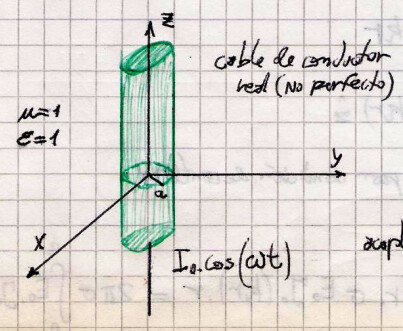
\includegraphics[width=0.3\textwidth]{images/fig_ft1_problema5_cuasiestac.jpg}

Se tiene 
\[
	\vb{J} = \sigma \vb{E},
	\label{corr_cable}
\]
donde $\sigma$ es constante. Digamos que en un cable la corriente
no circula igual en toda la sección, en corriente alterna. En corriente continua es uniforme.
Las ecuaciones de Maxwell de los campos eléctricos y magnéticos están acopladas como sabemos.
Clavándoles un rotor a ambas resulta
\notamargen{Esto tiene que estar hecho con detalle en el proóximo chapter.}
\[
	\nabla^2 \vb{E} + \Frac{\omega}{c}^2 \left( 1 + i \frac{4\pi\sigma}{\omega} \right) \vb{E} = 0,
\]
donde el factor lineal que multiplica al campo será denominado $K^2$. El campo $\vb E$ debe tener 
dirección en $\zver$ dado que la corriente tiene la dirección del campo. Se propone una solución
del tipo $ E_0 \euler^{i \omega t}$ y de la condición \eqref{corr_cable} vemos que el comportamiento
temporal tiene que ser del tipo propuesto.

En un buen conductor $\sigma$ es muy grande respecto de $\omega$; si ésta última crece deja de
ser un buen conductor. La aproximación de buen conductor implica entonces,
\[
	\frac{4 \omega \sigma }{\omega} \gg 1
\]
y utilizándola en nuestra ecuación para el campo eléctrico se tiene
\[
	K^2 \approx  i \frac{4\pi\sigma\omega}{c^2}
\]
y consecuentemente
\[
	K \frac{1+i}{\sqrt{2}} \frac{\sqrt{4 \pi \omega \sigma}}{c} = \frac{1+i}{\delta}
\]
donde 
\[
	\delta \equiv \frac{c}{\sqrt{2 \pi \omega \sigma}}
\]
tiene unidades de longitud y se denomina longitud de penetración. Será como una longitud
característica del problema dado que 
\[
	\delta = \frac{c}{\omega \sqrt{2 \pi \sigma / omega }}
\]
y entonces
\[
	\frac{\omega \delta }{c} \ll 1.
\]
Para resolver este problema aplicaremos el método cuasiestacionario.

{\bf Orden cero}.
Nos da sencillamente $\lapm{E}=0$.

{\bf Orden uno}.
Resulta la ecuación de Helmholtz para el campo eléctrico,
\[
	(\nabla^2+K^2 )\vb{E}^{(1)} = 0,
\]
que en coordenadas cilíndricas es la ecuación de Bessel, previo cambio de
variables a $x = Kr$,
\[
	\dtot[2]{\vb{E}^{(1)}}{x} + 
	\frac{1}{x}\dtot{\vb{E}^{(1)}}{x} + \vb{E}^{(1)} = 0
\]
su solución es 
\[
	\vb{E}^{(1)} = E_0 J_0(kr) \zver
\]
siendo $E_0$ una constante a determinar a partir de la condición de contorno.
Utilizando $\vb j$ para la corriente, para no confundir con las funciones de Bessel,
se tiene
\[
	I_0 = \int \vb j \: d\vb{S} = 
	2 \pi \sigma \int_0^a E_0 J_0(kr) r \: dr
\]
que se integrará con ayuda de las expresiones del apéndice \ref{apendice_bessel}.
Luego,
\[
	E_0 = \frac{I_0 K}{2 \pi \sigma a J_1(ka)}
\]
de manera que $E^{(1)} = E_0 J_0(kr)$.

De la ecuación del rotor del campo eléctrico se despeja el campo magnético hallándose
\[
	\vb{B}^{(0)} = - c \int E_0 J_1(kr) k \euler^{-i \omega t} \: dt \phiver, 
\]
de la cual se obtiene
\[
	\vb{B}^{(0)} = -\frac{icK}{\omega} \frac{I_0 K J_1(kr)}{2 \pi \sigma a J_1(ka)} 
	\euler^{-i \omega t} \phiver =
	\frac{2I_0}{ac} \frac{J_1(kr)}{J_1(ka)} \euler^{-i \omega t} \phiver
\]

Los siguientes grafiquetes muestran el comportamiento de $\vb j$ y de $\vb B$

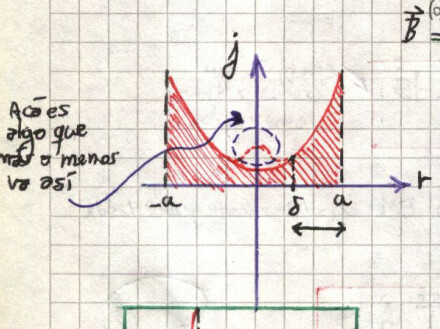
\includegraphics[width=0.4\textwidth]{images/fig_ft1_problema5_cuasiestacA.jpg}
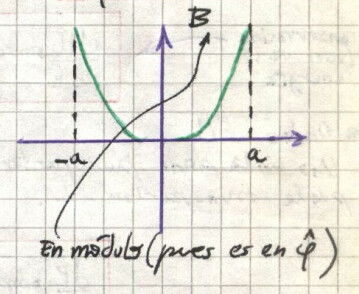
\includegraphics[width=0.4\textwidth]{images/fig_ft1_problema5_cuasiestacB.jpg}

donde se ve en función del radio y vemos que la corriente viaja casi por completo en las
paredes. Los casos límite se ven en estas ilustraciones.

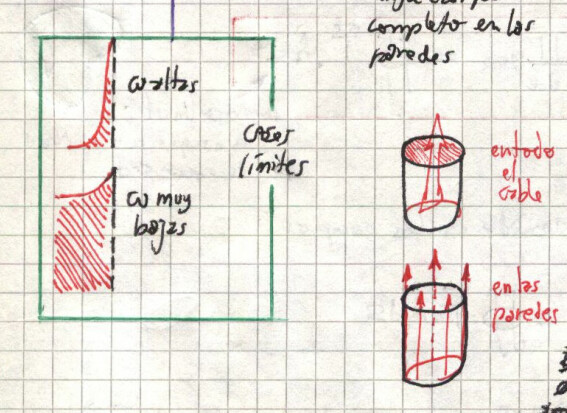
\includegraphics[width=0.4\textwidth]{images/fig_ft1_problema5_cuasiestacC.jpg}

Vemos también el cálculo del campo $\vb{B}$ afuera, mediante ley de Ampere,
\[
	B = \frac{2I_0}{ac} \Frac{r}{a}^2
\]
y su relación con las aproximaciones anteriores. Cuando $\omega$ es alta $B$ es nulo en el
interior.

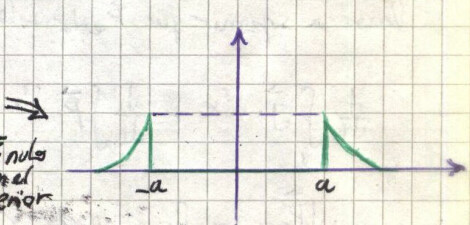
\includegraphics[width=0.4\textwidth]{images/fig_ft1_problema5_cuasiestacD.jpg}

Calculemos ahora la potencia disipada por efeco Joule. Será un cálculo de promedio temporal,
\[
	\langle \pe{J}{E}\rangle = \frac{1}{2} \mathcal{Re}\left\{ \vb J \cdot \vb E^* \right\}
\]
donde dentro de la toma de parte real son fasores. Entonces
\[
	\langle \pe{J}{E}\rangle = \frac{1}{2}\sigma 
	\mathcal{Re}\left\{ 
	\Frac{I_0 J_0(kr)}{2 \pi \sigma a |J_1(ka)|}^2 
	\frac{\sqrt{2}}{\delta} \euler^{i\pi/4} \euler^{i\omega t}
	\frac{\sqrt{2}}{\delta} \euler^{-i\pi/4} \euler^{i\omega t} \right\} =
	\frac{ I_0^2 |J_0(kr)|^2 }{ 4 \pi^2 \sigma a^2 |J_1(ka)|^2 \delta^2 }
\]

Esta es la disipación por unidad de volumen. Tenemos que integrar ahora
\[
	P = \int_0^{2\pi} d\phi \int_0^a r dr \int_0^L dz 
	\frac{ I_0^2 |J_0(kr)|^2 }{ 4 \pi^2 \sigma a^2 |J_1(ka)|^2 \delta^2 },
\]
y usando las propiedades de integración de las funciones de Bessel,
\[
	P = \frac{I_0^2}{4} \Frac{L}{\sigma \pi \delta^2 } \left( 1 + \frac{J_0(ka)}{J_1(ka)} \right)^2
\]
y como el paréntesis es $\sim 1$ se tiene que
\[
	P \approx \frac{I_0^2}{2} R_{\text{eq}}
\]
donde $ R_{\text{eq}} $ es una resistencia equivalente y la disipación se produce en la longitud
$\delta$ no en todo el radio del cable.
 
\end{ejemplo}


% \bibliographystyle{CBFT-apa-good}	% (uses file "apa-good.bst")
% \bibliography{CBFT.Referencias} % La base de datos bibliográfica

\end{document}
